% Options for packages loaded elsewhere
\PassOptionsToPackage{unicode}{hyperref}
\PassOptionsToPackage{hyphens}{url}
%
\documentclass[
]{article}
\usepackage{amsmath,amssymb}
\usepackage{lmodern}
\usepackage{iftex}
\ifPDFTeX
  \usepackage[T1]{fontenc}
  \usepackage[utf8]{inputenc}
  \usepackage{textcomp} % provide euro and other symbols
\else % if luatex or xetex
  \usepackage{unicode-math}
  \defaultfontfeatures{Scale=MatchLowercase}
  \defaultfontfeatures[\rmfamily]{Ligatures=TeX,Scale=1}
\fi
% Use upquote if available, for straight quotes in verbatim environments
\IfFileExists{upquote.sty}{\usepackage{upquote}}{}
\IfFileExists{microtype.sty}{% use microtype if available
  \usepackage[]{microtype}
  \UseMicrotypeSet[protrusion]{basicmath} % disable protrusion for tt fonts
}{}
\makeatletter
\@ifundefined{KOMAClassName}{% if non-KOMA class
  \IfFileExists{parskip.sty}{%
    \usepackage{parskip}
  }{% else
    \setlength{\parindent}{0pt}
    \setlength{\parskip}{6pt plus 2pt minus 1pt}}
}{% if KOMA class
  \KOMAoptions{parskip=half}}
\makeatother
\usepackage{xcolor}
\usepackage[margin=1in]{geometry}
\usepackage{color}
\usepackage{fancyvrb}
\newcommand{\VerbBar}{|}
\newcommand{\VERB}{\Verb[commandchars=\\\{\}]}
\DefineVerbatimEnvironment{Highlighting}{Verbatim}{commandchars=\\\{\}}
% Add ',fontsize=\small' for more characters per line
\usepackage{framed}
\definecolor{shadecolor}{RGB}{248,248,248}
\newenvironment{Shaded}{\begin{snugshade}}{\end{snugshade}}
\newcommand{\AlertTok}[1]{\textcolor[rgb]{0.94,0.16,0.16}{#1}}
\newcommand{\AnnotationTok}[1]{\textcolor[rgb]{0.56,0.35,0.01}{\textbf{\textit{#1}}}}
\newcommand{\AttributeTok}[1]{\textcolor[rgb]{0.77,0.63,0.00}{#1}}
\newcommand{\BaseNTok}[1]{\textcolor[rgb]{0.00,0.00,0.81}{#1}}
\newcommand{\BuiltInTok}[1]{#1}
\newcommand{\CharTok}[1]{\textcolor[rgb]{0.31,0.60,0.02}{#1}}
\newcommand{\CommentTok}[1]{\textcolor[rgb]{0.56,0.35,0.01}{\textit{#1}}}
\newcommand{\CommentVarTok}[1]{\textcolor[rgb]{0.56,0.35,0.01}{\textbf{\textit{#1}}}}
\newcommand{\ConstantTok}[1]{\textcolor[rgb]{0.00,0.00,0.00}{#1}}
\newcommand{\ControlFlowTok}[1]{\textcolor[rgb]{0.13,0.29,0.53}{\textbf{#1}}}
\newcommand{\DataTypeTok}[1]{\textcolor[rgb]{0.13,0.29,0.53}{#1}}
\newcommand{\DecValTok}[1]{\textcolor[rgb]{0.00,0.00,0.81}{#1}}
\newcommand{\DocumentationTok}[1]{\textcolor[rgb]{0.56,0.35,0.01}{\textbf{\textit{#1}}}}
\newcommand{\ErrorTok}[1]{\textcolor[rgb]{0.64,0.00,0.00}{\textbf{#1}}}
\newcommand{\ExtensionTok}[1]{#1}
\newcommand{\FloatTok}[1]{\textcolor[rgb]{0.00,0.00,0.81}{#1}}
\newcommand{\FunctionTok}[1]{\textcolor[rgb]{0.00,0.00,0.00}{#1}}
\newcommand{\ImportTok}[1]{#1}
\newcommand{\InformationTok}[1]{\textcolor[rgb]{0.56,0.35,0.01}{\textbf{\textit{#1}}}}
\newcommand{\KeywordTok}[1]{\textcolor[rgb]{0.13,0.29,0.53}{\textbf{#1}}}
\newcommand{\NormalTok}[1]{#1}
\newcommand{\OperatorTok}[1]{\textcolor[rgb]{0.81,0.36,0.00}{\textbf{#1}}}
\newcommand{\OtherTok}[1]{\textcolor[rgb]{0.56,0.35,0.01}{#1}}
\newcommand{\PreprocessorTok}[1]{\textcolor[rgb]{0.56,0.35,0.01}{\textit{#1}}}
\newcommand{\RegionMarkerTok}[1]{#1}
\newcommand{\SpecialCharTok}[1]{\textcolor[rgb]{0.00,0.00,0.00}{#1}}
\newcommand{\SpecialStringTok}[1]{\textcolor[rgb]{0.31,0.60,0.02}{#1}}
\newcommand{\StringTok}[1]{\textcolor[rgb]{0.31,0.60,0.02}{#1}}
\newcommand{\VariableTok}[1]{\textcolor[rgb]{0.00,0.00,0.00}{#1}}
\newcommand{\VerbatimStringTok}[1]{\textcolor[rgb]{0.31,0.60,0.02}{#1}}
\newcommand{\WarningTok}[1]{\textcolor[rgb]{0.56,0.35,0.01}{\textbf{\textit{#1}}}}
\usepackage{graphicx}
\makeatletter
\def\maxwidth{\ifdim\Gin@nat@width>\linewidth\linewidth\else\Gin@nat@width\fi}
\def\maxheight{\ifdim\Gin@nat@height>\textheight\textheight\else\Gin@nat@height\fi}
\makeatother
% Scale images if necessary, so that they will not overflow the page
% margins by default, and it is still possible to overwrite the defaults
% using explicit options in \includegraphics[width, height, ...]{}
\setkeys{Gin}{width=\maxwidth,height=\maxheight,keepaspectratio}
% Set default figure placement to htbp
\makeatletter
\def\fps@figure{htbp}
\makeatother
\setlength{\emergencystretch}{3em} % prevent overfull lines
\providecommand{\tightlist}{%
  \setlength{\itemsep}{0pt}\setlength{\parskip}{0pt}}
\setcounter{secnumdepth}{5}
\ifLuaTeX
  \usepackage{selnolig}  % disable illegal ligatures
\fi
\IfFileExists{bookmark.sty}{\usepackage{bookmark}}{\usepackage{hyperref}}
\IfFileExists{xurl.sty}{\usepackage{xurl}}{} % add URL line breaks if available
\urlstyle{same} % disable monospaced font for URLs
\hypersetup{
  pdftitle={HUDM6122 Homework\_01},
  pdfauthor={Chenguang Pan},
  hidelinks,
  pdfcreator={LaTeX via pandoc}}

\title{HUDM6122 Homework\_01}
\author{Chenguang Pan}
\date{Jan 28, 2023}

\begin{document}
\maketitle

\hypertarget{exercise-1.1}{%
\subsection{Exercise 1.1}\label{exercise-1.1}}

First, I made a xlsx. version of \texttt{Table\ 1.1} to let R read it
directly using the package `readxl``. This table is in 10x7 size. The
first column is just the index of each observation, so I drop it here.
Finally this dataset is in 9x7 size.

One should notice that the \texttt{sex}, \texttt{depression}, and
\texttt{health} are categorical variables. The Pearson Correlation
Coefficient is used for continuous rather than categorical variables.
Therefore, when calculate the correlation matrix we should drop the
categorical ones.

Note, there are some parameters need to be set. Since the original
dataset contains missing value, I construct the correlation matrix based
on all complete observations.

\begin{Shaded}
\begin{Highlighting}[]
\SpecialCharTok{\textgreater{}} \FunctionTok{library}\NormalTok{(readxl)}
\SpecialCharTok{\textgreater{}}\NormalTok{ table\_11 }\OtherTok{\textless{}{-}} \FunctionTok{read\_excel}\NormalTok{(}\StringTok{"table\_1.1.xlsx"}\NormalTok{)}
\SpecialCharTok{\textgreater{}}\NormalTok{ my\_data }\OtherTok{\textless{}{-}}\NormalTok{ table\_11[,}\FunctionTok{c}\NormalTok{(}\DecValTok{2}\SpecialCharTok{:}\DecValTok{7}\NormalTok{)]}
\SpecialCharTok{\textgreater{}} \CommentTok{\# drop the discrete vars and use only the complete observations}
\ErrorTok{\textgreater{}}\NormalTok{ my\_data\_cor }\OtherTok{\textless{}{-}} \FunctionTok{round}\NormalTok{(}\FunctionTok{cor}\NormalTok{(my\_data[,}\FunctionTok{c}\NormalTok{(}\DecValTok{2}\NormalTok{,}\DecValTok{3}\NormalTok{,}\DecValTok{6}\NormalTok{)], }\AttributeTok{use =} \StringTok{"complete"}\NormalTok{),}\DecValTok{2}\NormalTok{)}
\SpecialCharTok{\textgreater{}} \CommentTok{\# the output is rounded in two decimals.}
\ErrorTok{\textgreater{}}\NormalTok{ my\_data\_cor}
\NormalTok{         age    IQ weight}
\NormalTok{age     }\FloatTok{1.00} \SpecialCharTok{{-}}\FloatTok{0.15}  \SpecialCharTok{{-}}\FloatTok{0.12}
\NormalTok{IQ     }\SpecialCharTok{{-}}\FloatTok{0.15}  \FloatTok{1.00}   \FloatTok{0.75}
\NormalTok{weight }\SpecialCharTok{{-}}\FloatTok{0.12}  \FloatTok{0.75}   \FloatTok{1.00}
\end{Highlighting}
\end{Shaded}

\hypertarget{exercise-1.2}{%
\subsection{Exercise 1.2}\label{exercise-1.2}}

Fill the \texttt{NA} with the column's mean, and recalculate the
correlation matrix.

\begin{Shaded}
\begin{Highlighting}[]
\SpecialCharTok{\textgreater{}} \CommentTok{\# to impute the NA with mean using a for{-}loop}
\ErrorTok{\textgreater{}} \ControlFlowTok{for}\NormalTok{ (cols }\ControlFlowTok{in} \FunctionTok{c}\NormalTok{(}\DecValTok{2}\NormalTok{,}\DecValTok{3}\NormalTok{,}\DecValTok{6}\NormalTok{)) \{}
\SpecialCharTok{+}\NormalTok{   my\_data[,cols][}\FunctionTok{is.na}\NormalTok{(my\_data[,cols])] }\OtherTok{\textless{}{-}} \FunctionTok{mean}\NormalTok{(my\_data[,cols], }\AttributeTok{na.rm=}\NormalTok{T)}
\SpecialCharTok{+}\NormalTok{ \}}
\SpecialCharTok{\textgreater{}} \CommentTok{\# create the correlation matrix}
\ErrorTok{\textgreater{}}\NormalTok{ my\_data\_cor\_2 }\OtherTok{\textless{}{-}} \FunctionTok{round}\NormalTok{(}\FunctionTok{cor}\NormalTok{(my\_data[,}\FunctionTok{c}\NormalTok{(}\DecValTok{2}\NormalTok{,}\DecValTok{3}\NormalTok{,}\DecValTok{6}\NormalTok{)]),}\DecValTok{2}\NormalTok{)}
\SpecialCharTok{\textgreater{}}\NormalTok{ my\_data\_cor\_2 }
\NormalTok{         age    IQ weight}
\NormalTok{age     }\FloatTok{1.00} \SpecialCharTok{{-}}\FloatTok{0.14}  \SpecialCharTok{{-}}\FloatTok{0.10}
\NormalTok{IQ     }\SpecialCharTok{{-}}\FloatTok{0.14}  \FloatTok{1.00}   \FloatTok{0.52}
\NormalTok{weight }\SpecialCharTok{{-}}\FloatTok{0.10}  \FloatTok{0.52}   \FloatTok{1.00}
\end{Highlighting}
\end{Shaded}

\hypertarget{exercise-1.3}{%
\subsection{Exercise 1.3}\label{exercise-1.3}}

The authors may not clearly say where readers can find the original
dataset. After seeing the code underlying in this book's R package
\texttt{MVA}, and run this argument \texttt{demo("Ch-MVA")}, one can
find the \texttt{table\ 1.3}'s dataset information at the paragraph
named \texttt{code\ chunk\ number\ 5}. It is in another package called
\texttt{HSAUR2}. First, I draw the normal probability plots of each
variable.

\begin{Shaded}
\begin{Highlighting}[]
\SpecialCharTok{\textgreater{}} \CommentTok{\# load the Table 1.3\textquotesingle{}s original dataset }
\ErrorTok{\textgreater{}} \FunctionTok{library}\NormalTok{(HSAUR2)}
\SpecialCharTok{\textgreater{}} \CommentTok{\# dim(pottery)}
\ErrorTok{\textgreater{}} \CommentTok{\# names(pottery) \# the dataset is the same}
\ErrorTok{\textgreater{}} \CommentTok{\# layout(matrix(1:10, nc = 3))}
\ErrorTok{\textgreater{}} \FunctionTok{sapply}\NormalTok{(}\FunctionTok{colnames}\NormalTok{(pottery)[}\DecValTok{1}\SpecialCharTok{:}\DecValTok{9}\NormalTok{], }\ControlFlowTok{function}\NormalTok{(x)\{}
\SpecialCharTok{+}   \CommentTok{\# use double bracket can directly return the col}
\SpecialCharTok{+}   \FunctionTok{qqnorm}\NormalTok{(pottery[[x]], }\AttributeTok{main =}\NormalTok{ x)}
\SpecialCharTok{+}   \FunctionTok{qqline}\NormalTok{(pottery[[x]])}
\SpecialCharTok{+}\NormalTok{ \})}
\end{Highlighting}
\end{Shaded}

\$Al2O3 NULL

\$Fe2O3 NULL

\$MgO NULL

\$CaO NULL

\$Na2O NULL

\$K2O NULL

\$TiO2 NULL

\$MnO NULL

\$BaO NULL

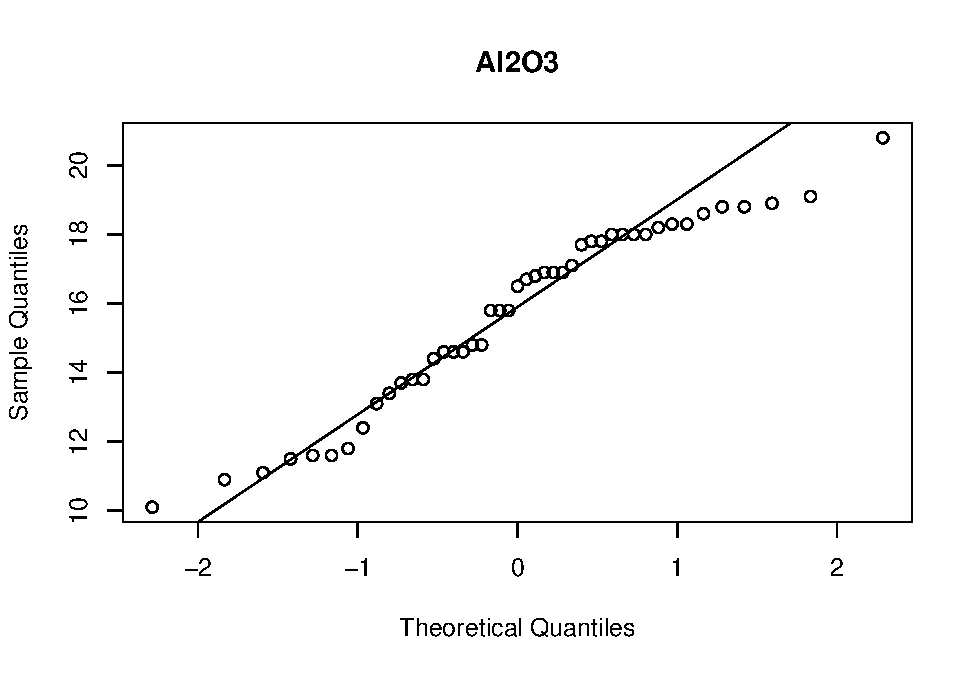
\includegraphics[width=0.33\linewidth,height=0.25\textheight]{hudm6122_hw_01_ChenguangPan_files/figure-latex/unnamed-chunk-3-1}
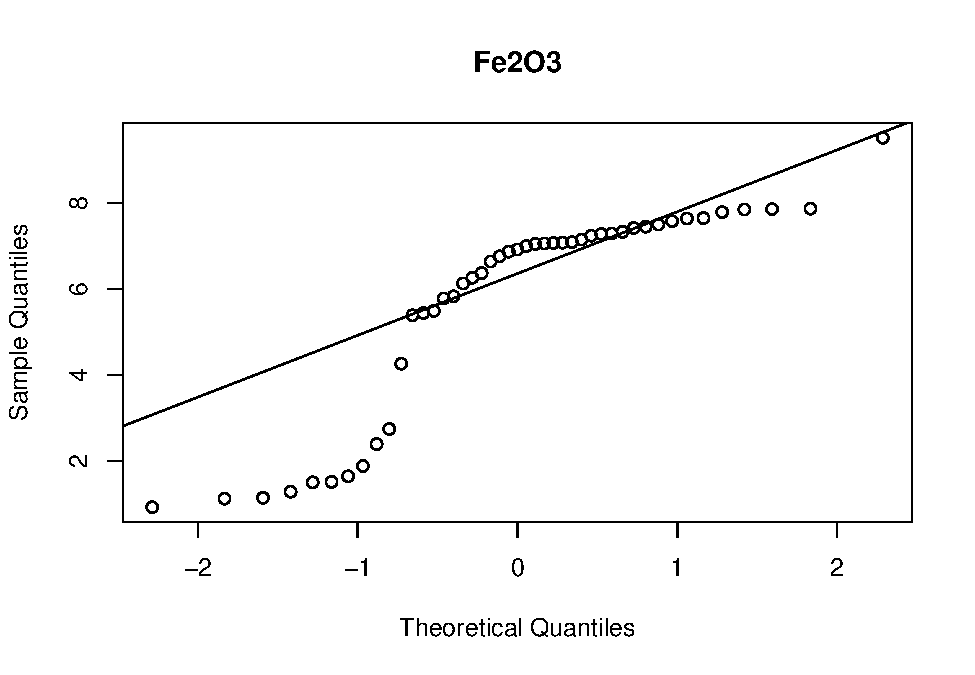
\includegraphics[width=0.33\linewidth,height=0.25\textheight]{hudm6122_hw_01_ChenguangPan_files/figure-latex/unnamed-chunk-3-2}
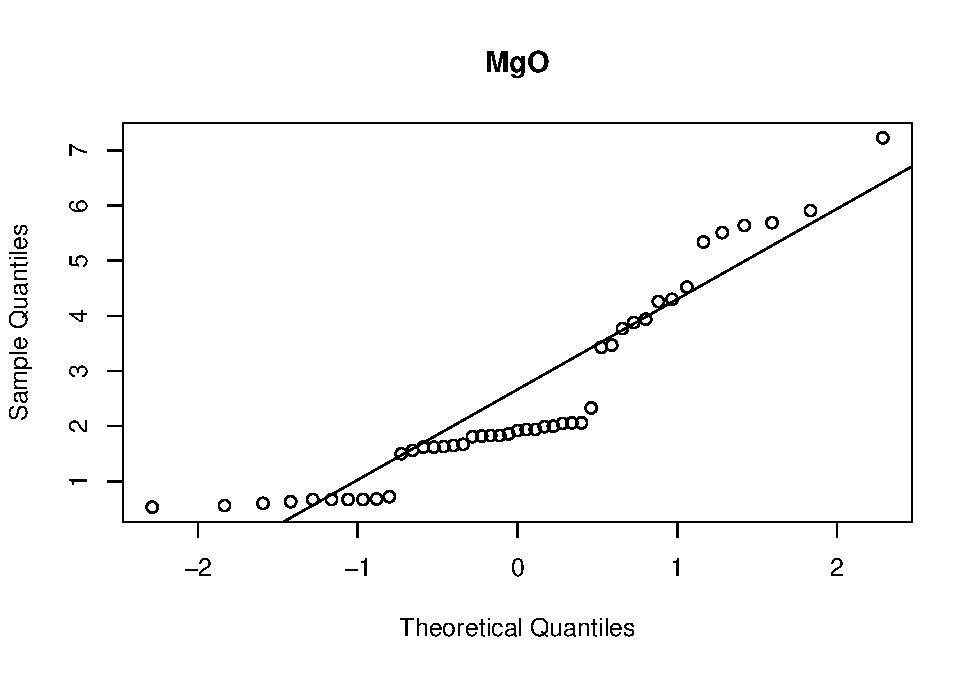
\includegraphics[width=0.33\linewidth,height=0.25\textheight]{hudm6122_hw_01_ChenguangPan_files/figure-latex/unnamed-chunk-3-3}
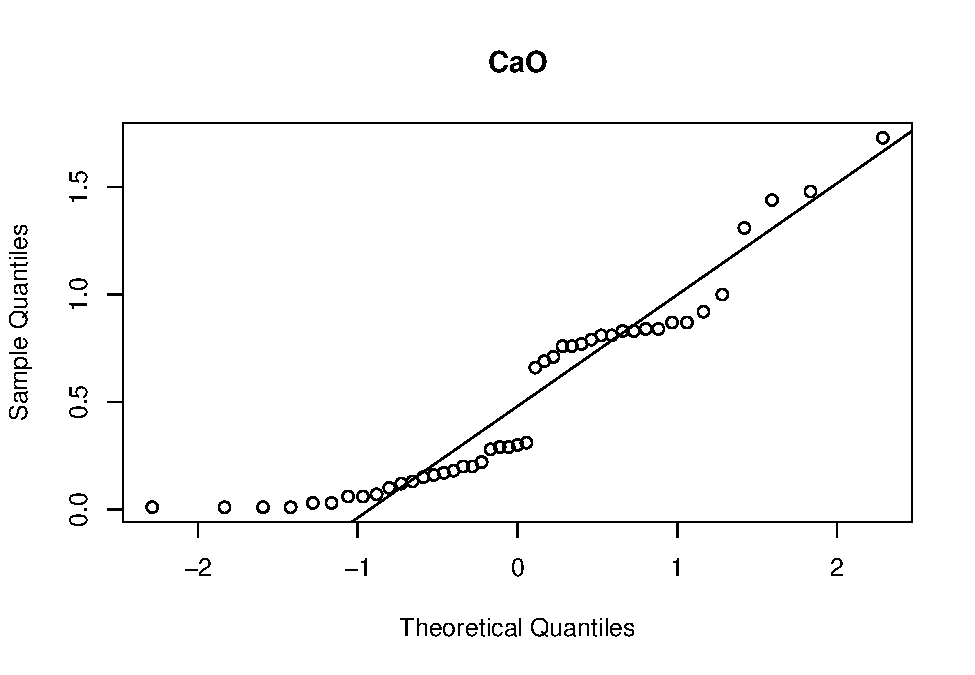
\includegraphics[width=0.33\linewidth,height=0.25\textheight]{hudm6122_hw_01_ChenguangPan_files/figure-latex/unnamed-chunk-3-4}
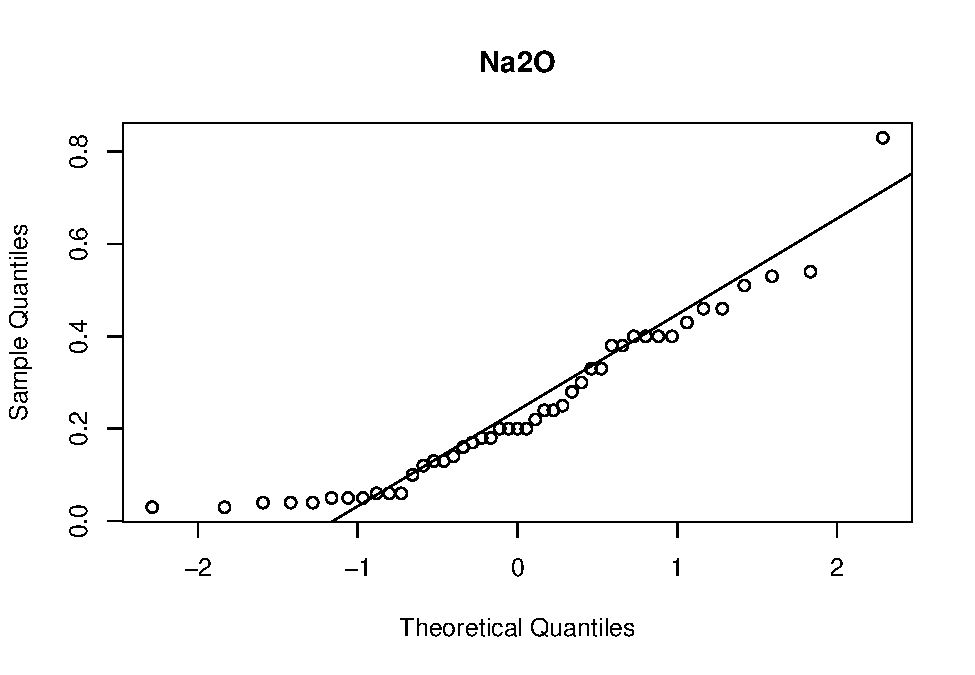
\includegraphics[width=0.33\linewidth,height=0.25\textheight]{hudm6122_hw_01_ChenguangPan_files/figure-latex/unnamed-chunk-3-5}
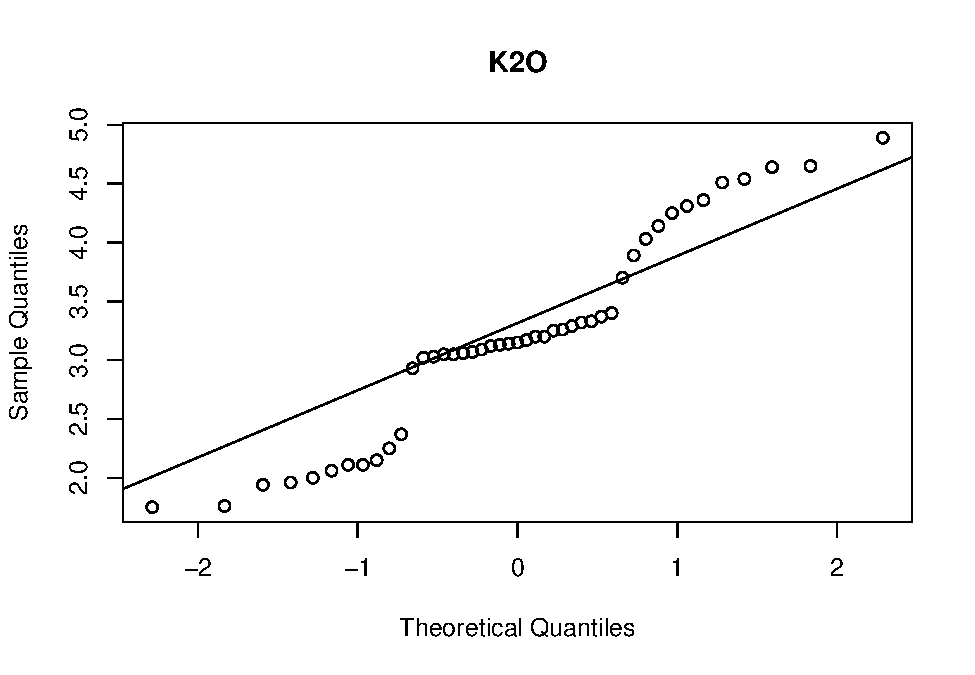
\includegraphics[width=0.33\linewidth,height=0.25\textheight]{hudm6122_hw_01_ChenguangPan_files/figure-latex/unnamed-chunk-3-6}
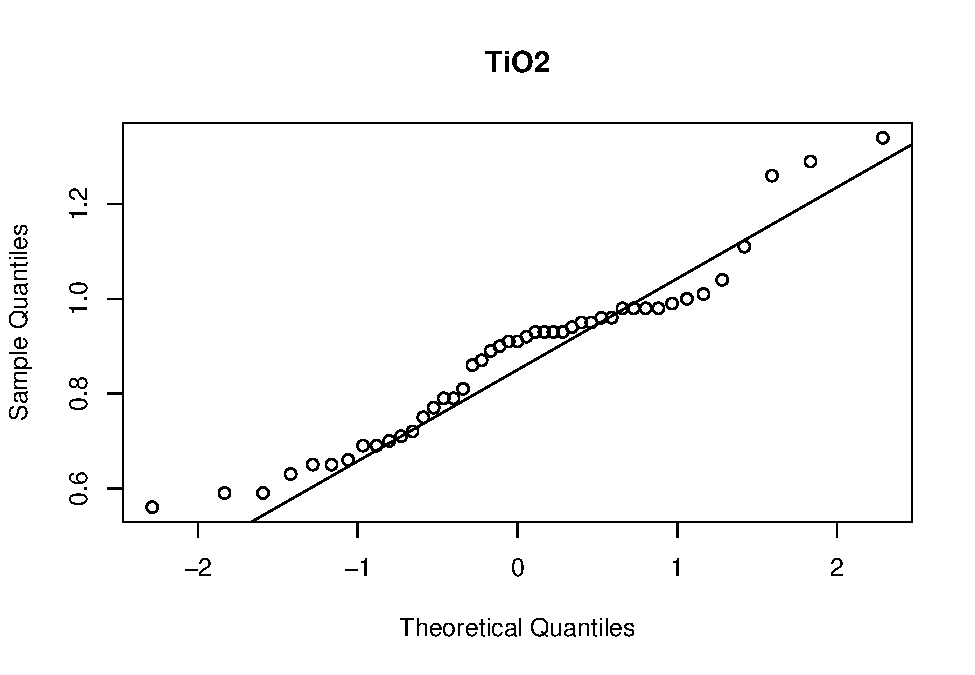
\includegraphics[width=0.33\linewidth,height=0.25\textheight]{hudm6122_hw_01_ChenguangPan_files/figure-latex/unnamed-chunk-3-7}
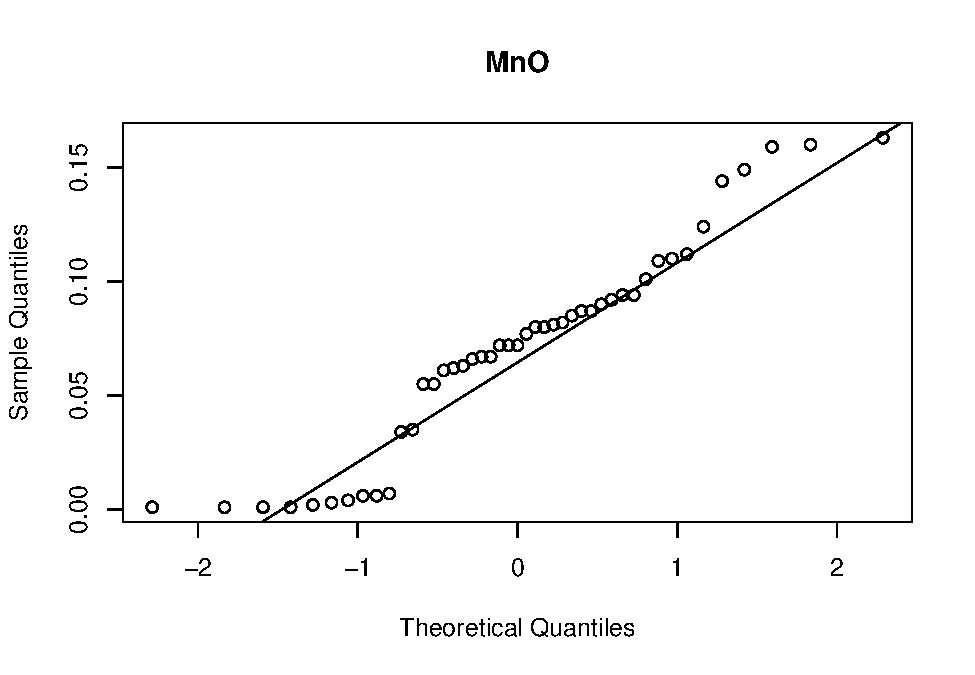
\includegraphics[width=0.33\linewidth,height=0.25\textheight]{hudm6122_hw_01_ChenguangPan_files/figure-latex/unnamed-chunk-3-8}
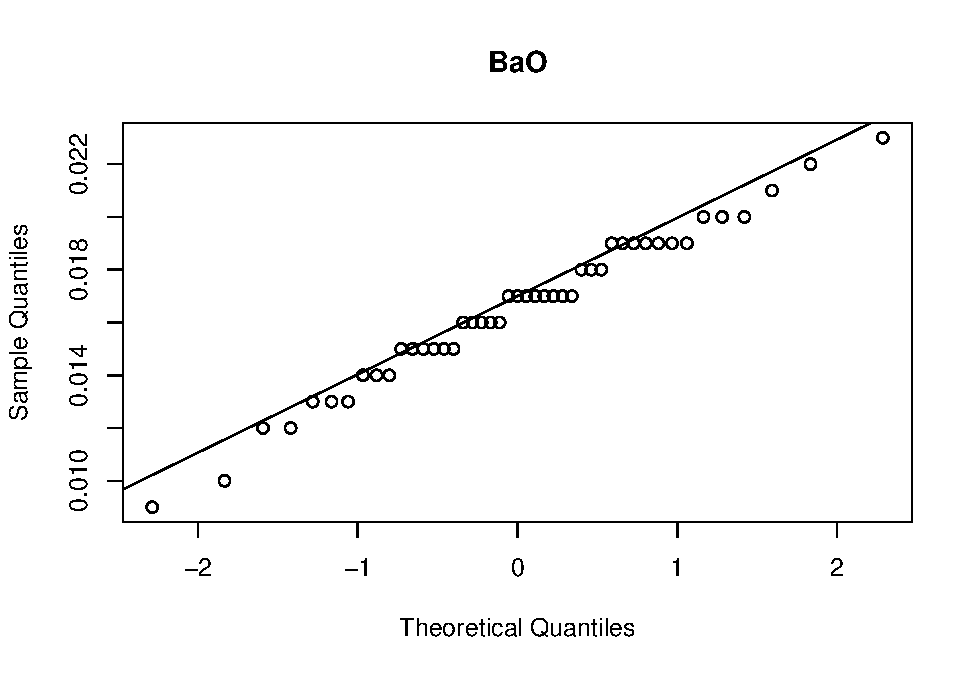
\includegraphics[width=0.33\linewidth,height=0.25\textheight]{hudm6122_hw_01_ChenguangPan_files/figure-latex/unnamed-chunk-3-9}
Second, I draw the chi-square plot of the data as followed.

\begin{Shaded}
\begin{Highlighting}[]
\SpecialCharTok{\textgreater{}} \CommentTok{\# to drop the last discrete variable}
\ErrorTok{\textgreater{}}\NormalTok{ X }\OtherTok{\textless{}{-}}\NormalTok{ pottery[,}\DecValTok{1}\SpecialCharTok{:}\DecValTok{9}\NormalTok{]}
\SpecialCharTok{\textgreater{}} \CommentTok{\# get each col\textquotesingle{}s mean}
\ErrorTok{\textgreater{}}\NormalTok{ col\_mean }\OtherTok{\textless{}{-}}  \FunctionTok{colMeans}\NormalTok{(X)}
\SpecialCharTok{\textgreater{}} \CommentTok{\# get the cov matrix}
\ErrorTok{\textgreater{}}\NormalTok{ S }\OtherTok{\textless{}{-}} \FunctionTok{cov}\NormalTok{(X)}
\SpecialCharTok{\textgreater{}} \CommentTok{\# solve() function can get inverse matrix directly}
\ErrorTok{\textgreater{}} \CommentTok{\# compute the generalised distance}
\ErrorTok{\textgreater{}}\NormalTok{ d }\OtherTok{\textless{}{-}} \FunctionTok{apply}\NormalTok{(X, }\DecValTok{1}\NormalTok{, }\CommentTok{\# array; 1= row 2 = col}
\SpecialCharTok{+}            \ControlFlowTok{function}\NormalTok{(X) }
\SpecialCharTok{+}              \FunctionTok{t}\NormalTok{(X }\SpecialCharTok{{-}}\NormalTok{ col\_mean) }\SpecialCharTok{\%*\%} \FunctionTok{solve}\NormalTok{(S) }\SpecialCharTok{\%*\%}\NormalTok{ (X }\SpecialCharTok{{-}}\NormalTok{ col\_mean))}
\SpecialCharTok{\textgreater{}} \FunctionTok{plot}\NormalTok{(qc }\OtherTok{\textless{}{-}} \FunctionTok{qchisq}\NormalTok{((}\DecValTok{1}\SpecialCharTok{:}\FunctionTok{nrow}\NormalTok{(X) }\SpecialCharTok{{-}} \DecValTok{1}\SpecialCharTok{/}\DecValTok{2}\NormalTok{)}\SpecialCharTok{/} \FunctionTok{nrow}\NormalTok{(X), }\AttributeTok{df =} \DecValTok{9}\NormalTok{),}
\SpecialCharTok{+}\NormalTok{      sd}\OtherTok{\textless{}{-}} \FunctionTok{sort}\NormalTok{(d),}
\SpecialCharTok{+}      \AttributeTok{xlab =} \FunctionTok{expression}\NormalTok{(}\FunctionTok{paste}\NormalTok{(chi[}\DecValTok{9}\NormalTok{]}\SpecialCharTok{\^{}}\DecValTok{2}\NormalTok{,}\StringTok{" Quantile"}\NormalTok{)),}
\SpecialCharTok{+}      \AttributeTok{ylab =} \StringTok{"Odered Distance"}\NormalTok{, }\AttributeTok{xlim =} \FunctionTok{range}\NormalTok{(qc)}\SpecialCharTok{*}\FunctionTok{c}\NormalTok{(}\DecValTok{1}\NormalTok{, }\FloatTok{1.1}\NormalTok{))}
\SpecialCharTok{\textgreater{}}\NormalTok{ oups }\OtherTok{\textless{}{-}} \FunctionTok{which}\NormalTok{(}\FunctionTok{rank}\NormalTok{(}\FunctionTok{abs}\NormalTok{(qc}\SpecialCharTok{{-}}\NormalTok{sd), }\AttributeTok{ties=}\StringTok{"random"}\NormalTok{) }\SpecialCharTok{\textgreater{}} \FunctionTok{nrow}\NormalTok{(X) }\SpecialCharTok{{-}} \DecValTok{3}\NormalTok{)}
\SpecialCharTok{\textgreater{}} \FunctionTok{text}\NormalTok{(qc[oups], sd[oups]}\SpecialCharTok{{-}}\FloatTok{1.5}\NormalTok{, }\FunctionTok{names}\NormalTok{(oups))}
\SpecialCharTok{\textgreater{}} \FunctionTok{abline}\NormalTok{(}\AttributeTok{a=}\DecValTok{0}\NormalTok{, }\AttributeTok{b=}\DecValTok{1}\NormalTok{)}
\end{Highlighting}
\end{Shaded}

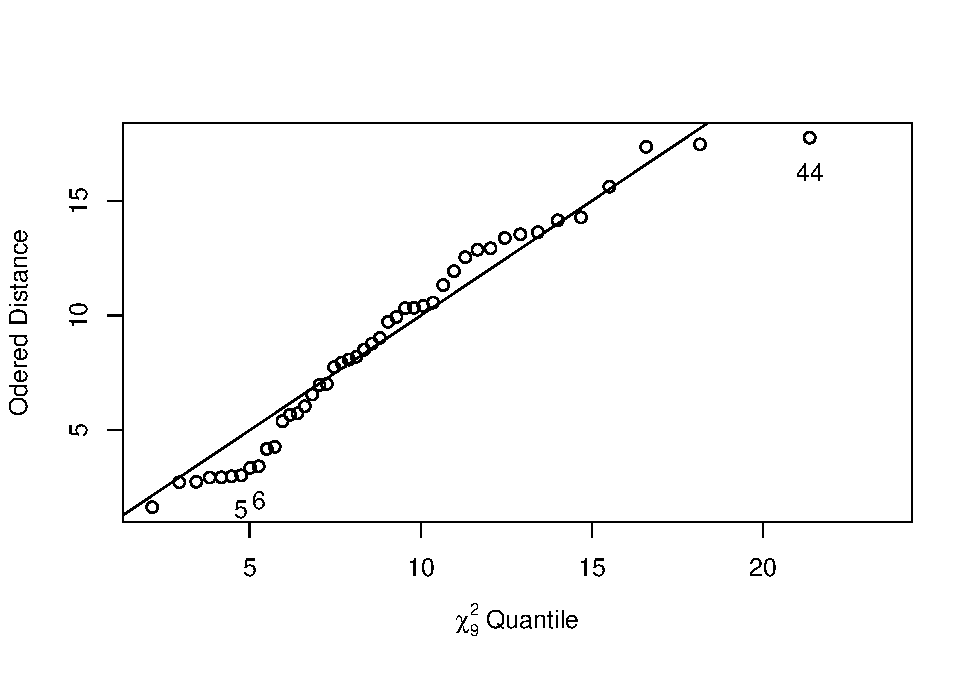
\includegraphics[width=0.5\linewidth,height=0.5\textheight]{hudm6122_hw_01_ChenguangPan_files/figure-latex/unnamed-chunk-4-1}

From the Q-Q plots, one can see most of the elements do not perfectly
follow the normal distribution except the \texttt{AL2O3} and the
\texttt{BaO} present relatively good normal distribution. As for the
Chi-square plot, if all the data are normally distributed, they should
correspond to each others. Therefore, from the plot, we can easily find
the outliers are the 5th, 6th, and the 44th observations.

\hypertarget{exercise-1.4}{%
\subsection{Exercise 1.4}\label{exercise-1.4}}

This question can be addressed in one line using \texttt{cov2cor}
function

\begin{Shaded}
\begin{Highlighting}[]
\SpecialCharTok{\textgreater{}} \CommentTok{\# import the cov matrix}
\ErrorTok{\textgreater{}}\NormalTok{ a\_matrix}\OtherTok{\textless{}{-}} \FunctionTok{matrix}\NormalTok{(}\FunctionTok{c}\NormalTok{(}\FloatTok{3.8778}\NormalTok{, }\FloatTok{2.8110}\NormalTok{, }\FloatTok{3.1480}\NormalTok{, }\FloatTok{3.5062}\NormalTok{,}
\SpecialCharTok{+}                     \FloatTok{2.8110}\NormalTok{, }\FloatTok{2.1210}\NormalTok{, }\FloatTok{2.2669}\NormalTok{, }\FloatTok{2.5690}\NormalTok{,}
\SpecialCharTok{+}                     \FloatTok{3.1480}\NormalTok{, }\FloatTok{2.2669}\NormalTok{, }\FloatTok{2.6550}\NormalTok{, }\FloatTok{2.8341}\NormalTok{,}
\SpecialCharTok{+}                     \FloatTok{3.5062}\NormalTok{, }\FloatTok{2.5690}\NormalTok{, }\FloatTok{2.8341}\NormalTok{, }\FloatTok{3.2352}\NormalTok{),}\DecValTok{4}\NormalTok{,}\DecValTok{4}\NormalTok{, }\AttributeTok{byrow=}\NormalTok{T)}
\SpecialCharTok{\textgreater{}} \FunctionTok{round}\NormalTok{(}\FunctionTok{cov2cor}\NormalTok{(a\_matrix),}\DecValTok{3}\NormalTok{)}
\NormalTok{      [,}\DecValTok{1}\NormalTok{]  [,}\DecValTok{2}\NormalTok{]  [,}\DecValTok{3}\NormalTok{]  [,}\DecValTok{4}\NormalTok{]}
\NormalTok{[}\DecValTok{1}\NormalTok{,] }\FloatTok{1.000} \FloatTok{0.980} \FloatTok{0.981} \FloatTok{0.990}
\NormalTok{[}\DecValTok{2}\NormalTok{,] }\FloatTok{0.980} \FloatTok{1.000} \FloatTok{0.955} \FloatTok{0.981}
\NormalTok{[}\DecValTok{3}\NormalTok{,] }\FloatTok{0.981} \FloatTok{0.955} \FloatTok{1.000} \FloatTok{0.967}
\NormalTok{[}\DecValTok{4}\NormalTok{,] }\FloatTok{0.990} \FloatTok{0.981} \FloatTok{0.967} \FloatTok{1.000}
\end{Highlighting}
\end{Shaded}

But here I provide another more specific code to achieve this goal.
Could you please consider to give me extra credits? Just kidding..lol..

\begin{Shaded}
\begin{Highlighting}[]
\SpecialCharTok{\textgreater{}} \CommentTok{\# function to convert covariance matrix to correlation matrix}
\ErrorTok{\textgreater{}}\NormalTok{ cov2cor\_test }\OtherTok{\textless{}{-}} \ControlFlowTok{function}\NormalTok{(covmat) \{}
\SpecialCharTok{+}\NormalTok{     sd\_vec }\OtherTok{\textless{}{-}} \FunctionTok{sqrt}\NormalTok{(}\FunctionTok{diag}\NormalTok{(covmat))}
\SpecialCharTok{+}\NormalTok{     cormat }\OtherTok{\textless{}{-}}\NormalTok{ covmat }\SpecialCharTok{/} \FunctionTok{outer}\NormalTok{(sd\_vec, sd\_vec)}
\SpecialCharTok{+}     \FunctionTok{return}\NormalTok{(cormat)}
\SpecialCharTok{+}\NormalTok{ \}}
\SpecialCharTok{\textgreater{}} 
\ErrorTok{\textgreater{}} \FunctionTok{round}\NormalTok{(}\FunctionTok{cov2cor\_test}\NormalTok{(a\_matrix),}\DecValTok{3}\NormalTok{)}
\NormalTok{      [,}\DecValTok{1}\NormalTok{]  [,}\DecValTok{2}\NormalTok{]  [,}\DecValTok{3}\NormalTok{]  [,}\DecValTok{4}\NormalTok{]}
\NormalTok{[}\DecValTok{1}\NormalTok{,] }\FloatTok{1.000} \FloatTok{0.980} \FloatTok{0.981} \FloatTok{0.990}
\NormalTok{[}\DecValTok{2}\NormalTok{,] }\FloatTok{0.980} \FloatTok{1.000} \FloatTok{0.955} \FloatTok{0.981}
\NormalTok{[}\DecValTok{3}\NormalTok{,] }\FloatTok{0.981} \FloatTok{0.955} \FloatTok{1.000} \FloatTok{0.967}
\NormalTok{[}\DecValTok{4}\NormalTok{,] }\FloatTok{0.990} \FloatTok{0.981} \FloatTok{0.967} \FloatTok{1.000}
\end{Highlighting}
\end{Shaded}

Finally, the results are exactly the same.

\hypertarget{exercise-1.5}{%
\subsection{Exercise 1.5}\label{exercise-1.5}}

\hypertarget{e1.5-part-1-create-the-euclidean-distance-matrix}{%
\subsubsection{E1.5 Part 1 Create the Euclidean Distance
Matrix}\label{e1.5-part-1-create-the-euclidean-distance-matrix}}

Here I write a function to get the Euclidean distance matrix for any
shape of observed matrix. Since for any m * n matrix, the size of
euclidean distance is always m * m.

\begin{Shaded}
\begin{Highlighting}[]
\SpecialCharTok{\textgreater{}} \CommentTok{\# write a function that can get Eu{-}dist matrix any shape of matrix}
\ErrorTok{\textgreater{}}\NormalTok{ eudis\_matrix }\OtherTok{\textless{}{-}} \ControlFlowTok{function}\NormalTok{(a\_matrix)\{}
\SpecialCharTok{+}   \CommentTok{\# first define a function to get the eu distance of any two vectors}
\SpecialCharTok{+}\NormalTok{   eu\_distance }\OtherTok{\textless{}{-}} \ControlFlowTok{function}\NormalTok{(vec\_1, vec\_2)\{}
\SpecialCharTok{+}\NormalTok{     d\_2\_vec }\OtherTok{\textless{}{-}}\NormalTok{ (vec\_1}\SpecialCharTok{{-}}\NormalTok{vec\_2)}\SpecialCharTok{\^{}}\DecValTok{2}
\SpecialCharTok{+}\NormalTok{     d\_2 }\OtherTok{\textless{}{-}} \FunctionTok{sum}\NormalTok{(d\_2\_vec)}
\SpecialCharTok{+}\NormalTok{     d }\OtherTok{\textless{}{-}} \FunctionTok{sqrt}\NormalTok{(d\_2)}
\SpecialCharTok{+}     \FunctionTok{return}\NormalTok{(d)}
\SpecialCharTok{+}\NormalTok{     \}}
\SpecialCharTok{+}   
\SpecialCharTok{+}\NormalTok{   m }\OtherTok{\textless{}{-}} \FunctionTok{nrow}\NormalTok{(a\_matrix)}
\SpecialCharTok{+}\NormalTok{   dist\_matrix }\OtherTok{\textless{}{-}} \FunctionTok{matrix}\NormalTok{(}\AttributeTok{nrow =}\NormalTok{ m, }\AttributeTok{ncol =}\NormalTok{ m)}
\SpecialCharTok{+}   \ControlFlowTok{for}\NormalTok{ (i }\ControlFlowTok{in} \DecValTok{1}\SpecialCharTok{:}\NormalTok{m ) \{}
\SpecialCharTok{+}     \ControlFlowTok{for}\NormalTok{ (j }\ControlFlowTok{in} \DecValTok{1}\SpecialCharTok{:}\NormalTok{m) \{}
\SpecialCharTok{+}\NormalTok{       dist\_matrix[i,j] }\OtherTok{\textless{}{-}} \FunctionTok{eu\_distance}\NormalTok{(a\_matrix[i,], a\_matrix[j,])}
\SpecialCharTok{+}\NormalTok{     \}}
\SpecialCharTok{+}\NormalTok{   \}}
\SpecialCharTok{+}   \FunctionTok{return}\NormalTok{(dist\_matrix)}
\SpecialCharTok{+}\NormalTok{ \}}
\end{Highlighting}
\end{Shaded}

The function seems good. Then, I tried it on the given dataset.

\begin{Shaded}
\begin{Highlighting}[]
\SpecialCharTok{\textgreater{}} \CommentTok{\# import the data}
\ErrorTok{\textgreater{}}\NormalTok{ multi\_mat}\OtherTok{\textless{}{-}} \FunctionTok{matrix}\NormalTok{(}\FunctionTok{c}\NormalTok{(}\DecValTok{3}\NormalTok{,}\DecValTok{6}\NormalTok{,}\DecValTok{4}\NormalTok{,}\DecValTok{0}\NormalTok{,}\DecValTok{7}\NormalTok{,}
\SpecialCharTok{+}                     \DecValTok{4}\NormalTok{,}\DecValTok{2}\NormalTok{,}\DecValTok{7}\NormalTok{,}\DecValTok{4}\NormalTok{,}\DecValTok{6}\NormalTok{,}
\SpecialCharTok{+}                     \DecValTok{4}\NormalTok{,}\DecValTok{0}\NormalTok{,}\DecValTok{3}\NormalTok{,}\DecValTok{1}\NormalTok{,}\DecValTok{5}\NormalTok{,}
\SpecialCharTok{+}                     \DecValTok{6}\NormalTok{,}\DecValTok{2}\NormalTok{,}\DecValTok{6}\NormalTok{,}\DecValTok{1}\NormalTok{,}\DecValTok{1}\NormalTok{,}
\SpecialCharTok{+}                     \DecValTok{1}\NormalTok{,}\DecValTok{6}\NormalTok{,}\DecValTok{2}\NormalTok{,}\DecValTok{1}\NormalTok{,}\DecValTok{4}\NormalTok{, }
\SpecialCharTok{+}                     \DecValTok{5}\NormalTok{,}\DecValTok{1}\NormalTok{,}\DecValTok{2}\NormalTok{,}\DecValTok{0}\NormalTok{,}\DecValTok{2}\NormalTok{,}
\SpecialCharTok{+}                     \DecValTok{1}\NormalTok{,}\DecValTok{1}\NormalTok{,}\DecValTok{2}\NormalTok{,}\DecValTok{6}\NormalTok{,}\DecValTok{1}\NormalTok{,}
\SpecialCharTok{+}                     \DecValTok{1}\NormalTok{,}\DecValTok{1}\NormalTok{,}\DecValTok{5}\NormalTok{,}\DecValTok{4}\NormalTok{,}\DecValTok{4}\NormalTok{,}
\SpecialCharTok{+}                     \DecValTok{7}\NormalTok{,}\DecValTok{0}\NormalTok{,}\DecValTok{1}\NormalTok{,}\DecValTok{3}\NormalTok{,}\DecValTok{3}\NormalTok{,}
\SpecialCharTok{+}                     \DecValTok{3}\NormalTok{,}\DecValTok{3}\NormalTok{,}\DecValTok{0}\NormalTok{,}\DecValTok{5}\NormalTok{,}\DecValTok{1}\NormalTok{),}\DecValTok{10}\NormalTok{,}\DecValTok{5}\NormalTok{, }\AttributeTok{byrow=}\NormalTok{T)}
\SpecialCharTok{\textgreater{}} \CommentTok{\# create the euclidean dis{-}matrix on the given dataset.}
\ErrorTok{\textgreater{}} \FunctionTok{round}\NormalTok{(}\FunctionTok{eudis\_matrix}\NormalTok{(multi\_mat),}\DecValTok{2}\NormalTok{)}
\NormalTok{       [,}\DecValTok{1}\NormalTok{] [,}\DecValTok{2}\NormalTok{] [,}\DecValTok{3}\NormalTok{] [,}\DecValTok{4}\NormalTok{] [,}\DecValTok{5}\NormalTok{] [,}\DecValTok{6}\NormalTok{]  [,}\DecValTok{7}\NormalTok{] [,}\DecValTok{8}\NormalTok{] [,}\DecValTok{9}\NormalTok{] [,}\DecValTok{10}\NormalTok{]}
\NormalTok{ [}\DecValTok{1}\NormalTok{,]  }\FloatTok{0.00} \FloatTok{6.56} \FloatTok{6.56} \FloatTok{8.12} \FloatTok{4.24} \FloatTok{7.62} \FloatTok{10.25} \FloatTok{7.42} \FloatTok{9.27}  \FloatTok{9.27}
\NormalTok{ [}\DecValTok{2}\NormalTok{,]  }\FloatTok{6.56} \FloatTok{0.00} \FloatTok{5.48} \FloatTok{6.24} \FloatTok{7.94} \FloatTok{7.68}  \FloatTok{8.00} \FloatTok{4.24} \FloatTok{7.68}  \FloatTok{8.77}
\NormalTok{ [}\DecValTok{3}\NormalTok{,]  }\FloatTok{6.56} \FloatTok{5.48} \FloatTok{0.00} \FloatTok{5.74} \FloatTok{6.86} \FloatTok{3.61}  \FloatTok{7.21} \FloatTok{4.90} \FloatTok{4.58}  \FloatTok{7.14}
\NormalTok{ [}\DecValTok{4}\NormalTok{,]  }\FloatTok{8.12} \FloatTok{6.24} \FloatTok{5.74} \FloatTok{0.00} \FloatTok{8.12} \FloatTok{4.47}  \FloatTok{8.19} \FloatTok{6.71} \FloatTok{6.16}  \FloatTok{7.87}
\NormalTok{ [}\DecValTok{5}\NormalTok{,]  }\FloatTok{4.24} \FloatTok{7.94} \FloatTok{6.86} \FloatTok{8.12} \FloatTok{0.00} \FloatTok{6.78}  \FloatTok{7.68} \FloatTok{6.56} \FloatTok{8.83}  \FloatTok{6.48}
\NormalTok{ [}\DecValTok{6}\NormalTok{,]  }\FloatTok{7.62} \FloatTok{7.68} \FloatTok{3.61} \FloatTok{4.47} \FloatTok{6.78} \FloatTok{0.00}  \FloatTok{7.28} \FloatTok{6.71} \FloatTok{4.00}  \FloatTok{6.16}
\NormalTok{ [}\DecValTok{7}\NormalTok{,] }\FloatTok{10.25} \FloatTok{8.00} \FloatTok{7.21} \FloatTok{8.19} \FloatTok{7.68} \FloatTok{7.28}  \FloatTok{0.00} \FloatTok{4.69} \FloatTok{7.14}  \FloatTok{3.61}
\NormalTok{ [}\DecValTok{8}\NormalTok{,]  }\FloatTok{7.42} \FloatTok{4.24} \FloatTok{4.90} \FloatTok{6.71} \FloatTok{6.56} \FloatTok{6.71}  \FloatTok{4.69} \FloatTok{0.00} \FloatTok{7.42}  \FloatTok{6.56}
\NormalTok{ [}\DecValTok{9}\NormalTok{,]  }\FloatTok{9.27} \FloatTok{7.68} \FloatTok{4.58} \FloatTok{6.16} \FloatTok{8.83} \FloatTok{4.00}  \FloatTok{7.14} \FloatTok{7.42} \FloatTok{0.00}  \FloatTok{5.83}
\NormalTok{[}\DecValTok{10}\NormalTok{,]  }\FloatTok{9.27} \FloatTok{8.77} \FloatTok{7.14} \FloatTok{7.87} \FloatTok{6.48} \FloatTok{6.16}  \FloatTok{3.61} \FloatTok{6.56} \FloatTok{5.83}  \FloatTok{0.00}
\end{Highlighting}
\end{Shaded}

Note each row of an empirical data n*p matrix represents an
observation/vector with P dimensions. Therefore, the entry{[}i, j{]} on
a n*n Euclidean distance matrix must be a scalar rather than a vector
and represents the euclidean distance between ith observation/vector and
jth observation/vector.

\hypertarget{e1.5-part-2-create-the-city-block-distance-matrix}{%
\subsubsection{E1.5 Part 2 Create the City Block Distance
Matrix}\label{e1.5-part-2-create-the-city-block-distance-matrix}}

Here this question raise alternative concept called
\texttt{city\ block\ distance}. It is the sum of the absolute
differences of the blocks' coordinates.

\begin{Shaded}
\begin{Highlighting}[]
\SpecialCharTok{\textgreater{}} \CommentTok{\# write a function that can get city block distance}
\ErrorTok{\textgreater{}}\NormalTok{ city\_matrix}\OtherTok{\textless{}{-}}\ControlFlowTok{function}\NormalTok{(a\_matrix)\{}
\SpecialCharTok{+}   \CommentTok{\# first define a function to get the eu distance of any two vectors}
\SpecialCharTok{+}\NormalTok{   city\_distance }\OtherTok{\textless{}{-}} \ControlFlowTok{function}\NormalTok{(vec\_1, vec\_2)\{}
\SpecialCharTok{+}\NormalTok{     city\_dist }\OtherTok{\textless{}{-}} \FunctionTok{sum}\NormalTok{(}\FunctionTok{abs}\NormalTok{(vec\_1}\SpecialCharTok{{-}}\NormalTok{vec\_2))}
\SpecialCharTok{+}     \FunctionTok{return}\NormalTok{(city\_dist)}
\SpecialCharTok{+}\NormalTok{     \}}
\SpecialCharTok{+}   
\SpecialCharTok{+}\NormalTok{   m }\OtherTok{\textless{}{-}} \FunctionTok{nrow}\NormalTok{(a\_matrix)}
\SpecialCharTok{+}\NormalTok{   c\_matrix }\OtherTok{\textless{}{-}} \FunctionTok{matrix}\NormalTok{(}\AttributeTok{nrow =}\NormalTok{ m, }\AttributeTok{ncol =}\NormalTok{ m)}
\SpecialCharTok{+}   \ControlFlowTok{for}\NormalTok{ (i }\ControlFlowTok{in} \DecValTok{1}\SpecialCharTok{:}\NormalTok{m ) \{}
\SpecialCharTok{+}     \ControlFlowTok{for}\NormalTok{ (j }\ControlFlowTok{in} \DecValTok{1}\SpecialCharTok{:}\NormalTok{m) \{}
\SpecialCharTok{+}\NormalTok{       c\_matrix[i,j] }\OtherTok{\textless{}{-}} \FunctionTok{city\_distance}\NormalTok{(a\_matrix[i,], a\_matrix[j,])}
\SpecialCharTok{+}\NormalTok{     \}}
\SpecialCharTok{+}\NormalTok{   \}}
\SpecialCharTok{+}   \FunctionTok{return}\NormalTok{(c\_matrix)}
\SpecialCharTok{+}\NormalTok{ \}}
\end{Highlighting}
\end{Shaded}

This function seems to work well. Try it on the given data:

\begin{Shaded}
\begin{Highlighting}[]
\SpecialCharTok{\textgreater{}} \FunctionTok{city\_matrix}\NormalTok{(multi\_mat)}
\NormalTok{      [,}\DecValTok{1}\NormalTok{] [,}\DecValTok{2}\NormalTok{] [,}\DecValTok{3}\NormalTok{] [,}\DecValTok{4}\NormalTok{] [,}\DecValTok{5}\NormalTok{] [,}\DecValTok{6}\NormalTok{] [,}\DecValTok{7}\NormalTok{] [,}\DecValTok{8}\NormalTok{] [,}\DecValTok{9}\NormalTok{] [,}\DecValTok{10}\NormalTok{]}
\NormalTok{ [}\DecValTok{1}\NormalTok{,]    }\DecValTok{0}   \DecValTok{13}   \DecValTok{11}   \DecValTok{16}    \DecValTok{8}   \DecValTok{14}   \DecValTok{21}   \DecValTok{15}   \DecValTok{20}    \DecValTok{18}
\NormalTok{ [}\DecValTok{2}\NormalTok{,]   }\DecValTok{13}    \DecValTok{0}   \DecValTok{10}   \DecValTok{11}   \DecValTok{17}   \DecValTok{15}   \DecValTok{16}    \DecValTok{8}   \DecValTok{15}    \DecValTok{15}
\NormalTok{ [}\DecValTok{3}\NormalTok{,]   }\DecValTok{11}   \DecValTok{10}    \DecValTok{0}   \DecValTok{11}   \DecValTok{11}    \DecValTok{7}   \DecValTok{14}   \DecValTok{10}    \DecValTok{9}    \DecValTok{15}
\NormalTok{ [}\DecValTok{4}\NormalTok{,]   }\DecValTok{16}   \DecValTok{11}   \DecValTok{11}    \DecValTok{0}   \DecValTok{16}    \DecValTok{8}   \DecValTok{15}   \DecValTok{13}   \DecValTok{12}    \DecValTok{14}
\NormalTok{ [}\DecValTok{5}\NormalTok{,]    }\DecValTok{8}   \DecValTok{17}   \DecValTok{11}   \DecValTok{16}    \DecValTok{0}   \DecValTok{12}   \DecValTok{13}   \DecValTok{11}   \DecValTok{16}    \DecValTok{14}
\NormalTok{ [}\DecValTok{6}\NormalTok{,]   }\DecValTok{14}   \DecValTok{15}    \DecValTok{7}    \DecValTok{8}   \DecValTok{12}    \DecValTok{0}   \DecValTok{11}   \DecValTok{13}    \DecValTok{8}    \DecValTok{12}
\NormalTok{ [}\DecValTok{7}\NormalTok{,]   }\DecValTok{21}   \DecValTok{16}   \DecValTok{14}   \DecValTok{15}   \DecValTok{13}   \DecValTok{11}    \DecValTok{0}    \DecValTok{8}   \DecValTok{13}     \DecValTok{7}
\NormalTok{ [}\DecValTok{8}\NormalTok{,]   }\DecValTok{15}    \DecValTok{8}   \DecValTok{10}   \DecValTok{13}   \DecValTok{11}   \DecValTok{13}    \DecValTok{8}    \DecValTok{0}   \DecValTok{13}    \DecValTok{13}
\NormalTok{ [}\DecValTok{9}\NormalTok{,]   }\DecValTok{20}   \DecValTok{15}    \DecValTok{9}   \DecValTok{12}   \DecValTok{16}    \DecValTok{8}   \DecValTok{13}   \DecValTok{13}    \DecValTok{0}    \DecValTok{12}
\NormalTok{[}\DecValTok{10}\NormalTok{,]   }\DecValTok{18}   \DecValTok{15}   \DecValTok{15}   \DecValTok{14}   \DecValTok{14}   \DecValTok{12}    \DecValTok{7}   \DecValTok{13}   \DecValTok{12}     \DecValTok{0}
\end{Highlighting}
\end{Shaded}


\end{document}
